\definecolor{hypnosVol}{HTML}{ffefba}
\definecolor{hypnosNonVol}{HTML}{87bfc7}

\subsection{Heterogeneous Cache Simulation} \label{sec:nvm-cache}

\subsubsection{Overview}


 
  
   
    
    
    


Particularly for the area of embedded systems, the SRAM technology conventionally used for cache memories has a number of sub-optimal properties.
Namely, SRAM cells are very space inefficient and incorporate a high static power consumption.
As mentioned in \cref{sec:commercial_maturity}, non-volatile STT-RAM is a promising alternative to SRAM, due to its low static power and high density allowing for smaller chip designs.
Nevertheless, a pure STT-RAM cache will likely suffer from high write overhead and cost.
Instead, a hybrid cache combining both SRAM and STT-RAM is a promising direction \cite{4798259,5090762,7479181,9399236}.  In this case study, we present a tool to evaluate different configurations of hybrid cache designs.









\subsubsection{Objective}
\cref{fig:FAU-archOverview} illustrates the memory hierarchy of the analyzed system, with a PCM-based main memory connected to the CPU via a hybrid cache.
This study examines how the SRAM-to-STT-RAM ratio in the hybrid cache affects dynamic energy consumption and overall latency across various embedded applications.
The goal is to provide insights for designing an optimal ratio tailored to specific application requirements.

\begin{figure}[h]
    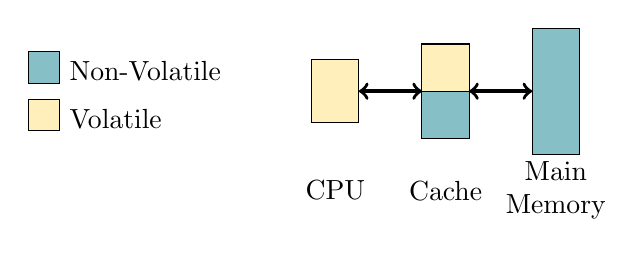
\begin{tikzpicture}[scale=0.4]
\path (11.75,-1.65) node[align = center] (dram) {Main\\Memory};
\path (8.25,-1.65) node[align = center] (cache) {Cache};
\path (4.75,-1.65) node[align = center] (cpu) {CPU};




\draw[fill = hypnosNonVol] (11,-0.5) rectangle (12.5,3.5);
\draw[fill = hypnosVol] (4,0.5) rectangle (5.5,2.5);



\draw[fill = hypnosVol] (7.5,1.5) rectangle (9,3);
\draw[fill = hypnosNonVol] (7.5,0) rectangle (9,1.5);

\draw[<->, line width = 1.25 pt] (5.5,1.5)--(7.5,1.5);
\draw[<->, line width = 1.25 pt] (9,1.5)--(11,1.5);

%----- legend
\draw[fill=hypnosVol] (-5,0.25) rectangle (-4,1.25) node[align = left, below right] () {Volatile};
\draw[fill=hypnosNonVol] (-5,1.75) rectangle (-4,2.75) node[align = left, below right] () {Non-Volatile};

\end{tikzpicture}
    \caption{Overview of the hybrid volatile/non-volatile memory hierarchies analyzed in this case study.}
    \label{fig:FAU-archOverview}
\end{figure}

   
  


\subsubsection{Methodology}

As gem5 does not support any hybrid caches out of the box, the following extensions were necessary.
a) STT-RAM cells have different access latencies, depending on whether a cell is read or written, with write latencies being higher as the orientation of the magnetic field has to be changed when switching the content of a cell.
Therefore, the simulator naturally had to be extended to feature asymmetric STT-RAM access latencies, along the (symmetric) access latency for SRAM cells.
b) Furthermore, the simulator was extended to generate a number of statistics specific to hybrid caches in order to give key insights into the experimental results.
Most importantly, we have added statistics to count the number of accesses, further split between read and write accesses, to each of the two cache sections, namely the volatile SRAM and the non-volatile STT-RAM section.
This access distribution can not only be used for the analysis of cache access patterns, but is also used to calculate the dynamic energy consumption caused by accesses to the different sections of the cache.
\par
As mentioned in the previous section, the degree to which non-volatility is introduced to the cache hierarchy is a key point of our analysis.
To be precise, the hybridization of the caches takes place on cache set level.
The cache set where requested data is potentially located is determined by the address of the request.
In an $n$-way associative cache, implementing $n_0$ cache lines per set in SRAM and $n_1$ cache lines in STT-RAM technology, wrt. $n_0 + n_1 = n$, thus allows for data to be placed in either the SRAM or the STT-RAM section.
In order to evaluate hybrid caches with different degrees of non-volatility, we have added a parameter called \texttt{nvBlockRatio} which sets the percentage of cache lines per set that are simulated as being implemented in the non-volatile STT-RAM technology, i.e., $n_1 = \left\lfloor\frac{\text{\texttt{nvBlockRatio}}}{100} \cdot n\right\rfloor$.
The effect of different \texttt{nvBlockRatio} settings on the configuration can be seen in \cref{fig:FAU-nvBlockratio}
\begin{figure}
    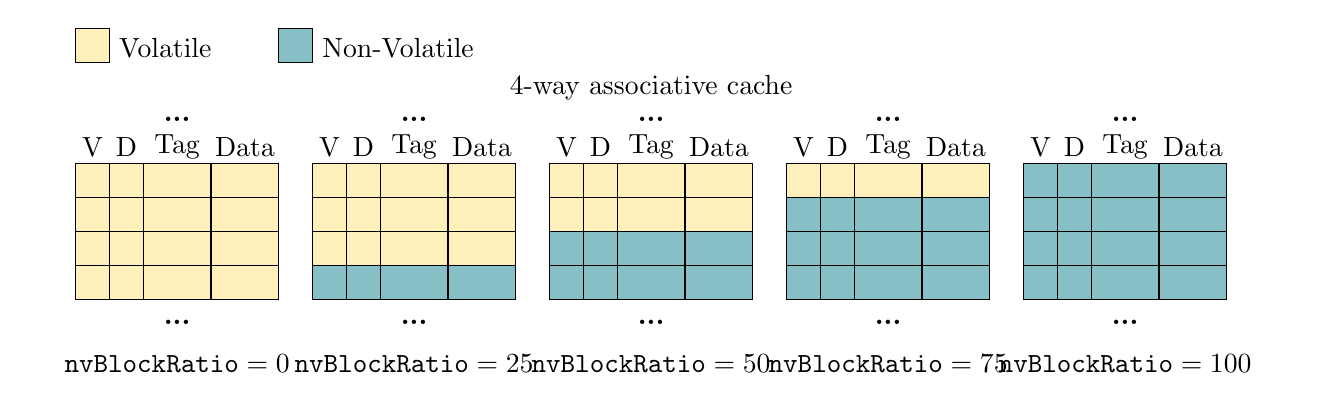
\begin{tikzpicture}[scale = 0.43]

%----- sample set
\path (1+14,7.25) node[align = center] () {4-way associative cache};

\path (1,6.3) node[align = center] () {\textbf{...}};
\path (1,0.3) node[align = center] () {\textbf{...}};

\path (-1.5,5.5) node[align = center] (vb) {\phantom{|}V\phantom{|}};
\path (-0.5,5.5) node[align = center] (db) {\phantom{|}D\phantom{|}};
\path (1,5.5) node[align = center] (tag) {\phantom{|}Tag\phantom{|}};
\path (3,5.5) node[align = center] (data) {\phantom{|}Data\phantom{|}};

\draw [fill = hypnosVol]  (-2,4) rectangle (-1,5);
\draw [fill = hypnosVol] (-1,4) rectangle (0,5);
\draw [fill = hypnosVol] (0,4) rectangle (2,5);
\draw [fill = hypnosVol]  (2,4) rectangle (4,5);

\draw [fill = hypnosVol]  (-2,3) rectangle (-1,4);
\draw [fill = hypnosVol] (-1,3) rectangle (0,4);
\draw [fill = hypnosVol]  (0,3) rectangle (2,4);
\draw [fill = hypnosVol]  (2,3) rectangle (4,4);

\draw [fill = hypnosVol]  (-2,2) rectangle (-1,3);
\draw [fill = hypnosVol]  (-1,2) rectangle (0,3);
\draw [fill = hypnosVol]  (0,2) rectangle (2,3);
\draw [fill = hypnosVol]  (2,2) rectangle (4,3);

\draw [fill = hypnosVol]  (-2,1) rectangle (-1,2);
\draw [fill = hypnosVol]  (-1,1) rectangle (0,2);
\draw [fill = hypnosVol]  (0,1) rectangle (2,2);
\draw [fill = hypnosVol]  (2,1) rectangle (4,2);


%--------

\path (1+7,6.3) node[align = center] () {\textbf{...}};
\path (1+7,0.3) node[align = center] () {\textbf{...}};

\path (5.5,5.5) node[align = center] (vb) {\phantom{|}V\phantom{|}};
\path (6.5,5.5) node[align = center] (db) {\phantom{|}D\phantom{|}};
\path (8,5.5) node[align = center] (tag) {\phantom{|}Tag\phantom{|}};
\path (10,5.5) node[align = center] (data) {\phantom{|}Data\phantom{|}};

\draw [fill = hypnosVol]  (5,4) rectangle (6,5);
\draw [fill = hypnosVol] (6,4) rectangle (7,5);
\draw [fill = hypnosVol] (7,4) rectangle (9,5);
\draw [fill = hypnosVol]  (9,4) rectangle (11,5);

\draw [fill = hypnosVol]  (5,3) rectangle (6,4);
\draw [fill = hypnosVol] (6,3) rectangle (7,4);
\draw [fill = hypnosVol]  (7,3) rectangle (9,4);
\draw [fill = hypnosVol]  (9,3) rectangle (11,4);

\draw [fill = hypnosVol]  (5,2) rectangle (6,3);
\draw [fill = hypnosVol]  (6,2) rectangle (7,3);
\draw [fill = hypnosVol]  (7,2) rectangle (9,3);
\draw [fill = hypnosVol]  (9,2) rectangle (11,3);

\draw [fill = hypnosNonVol]  (5,1) rectangle (6,2);
\draw [fill = hypnosNonVol]  (6,1) rectangle (7,2);
\draw [fill = hypnosNonVol]  (7,1) rectangle (9,2);
\draw [fill = hypnosNonVol]  (9,1) rectangle (11,2);


%--------

\path (1+14,6.3) node[align = center] () {\textbf{...}};
\path (1+14,0.3) node[align = center] () {\textbf{...}};

\path (12.5,5.5) node[align = center] (vb) {\phantom{|}V\phantom{|}};
\path (13.5,5.5) node[align = center] (db) {\phantom{|}D\phantom{|}};
\path (15,5.5) node[align = center] (tag) {\phantom{|}Tag\phantom{|}};
\path (17,5.5) node[align = center] (data) {\phantom{|}Data\phantom{|}};

\draw [fill = hypnosVol]  (12,4) rectangle (13,5);
\draw [fill = hypnosVol] (13,4) rectangle (14,5);
\draw [fill = hypnosVol] (14,4) rectangle (16,5);
\draw [fill = hypnosVol]  (16,4) rectangle (18,5);

\draw [fill = hypnosVol]  (12,3) rectangle (13,4);
\draw [fill = hypnosVol] (13,3) rectangle (14,4);
\draw [fill = hypnosVol]  (14,3) rectangle (16,4);
\draw [fill = hypnosVol]  (16,3) rectangle (18,4);

\draw [fill = hypnosNonVol]  (12,2) rectangle (13,3);
\draw [fill = hypnosNonVol]  (13,2) rectangle (14,3);
\draw [fill = hypnosNonVol]  (14,2) rectangle (16,3);
\draw [fill = hypnosNonVol]  (16,2) rectangle (18,3);

\draw [fill = hypnosNonVol]  (12,1) rectangle (13,2);
\draw [fill = hypnosNonVol]  (13,1) rectangle (14,2);
\draw [fill = hypnosNonVol]  (14,1) rectangle (16,2);
\draw [fill = hypnosNonVol]  (16,1) rectangle (18,2);


%--------

\path (1+21,6.3) node[align = center] () {\textbf{...}};
\path (1+21,0.3) node[align = center] () {\textbf{...}};

\path (19.5,5.5) node[align = center] (vb) {\phantom{|}V\phantom{|}};
\path (20.5,5.5) node[align = center] (db) {\phantom{|}D\phantom{|}};
\path (22,5.5) node[align = center] (tag) {\phantom{|}Tag\phantom{|}};
\path (24,5.5) node[align = center] (data) {\phantom{|}Data\phantom{|}};

\draw [fill = hypnosVol]  (7+12,4) rectangle (7+13,5);
\draw [fill = hypnosVol] (7+13,4) rectangle (7+14,5);
\draw [fill = hypnosVol] (7+14,4) rectangle (7+16,5);
\draw [fill = hypnosVol]  (7+16,4) rectangle (7+18,5);

\draw [fill = hypnosNonVol]  (7+12,3) rectangle (7+13,4);
\draw [fill = hypnosNonVol] (7+13,3) rectangle (7+14,4);
\draw [fill = hypnosNonVol]  (7+14,3) rectangle (7+16,4);
\draw [fill = hypnosNonVol]  (7+16,3) rectangle (7+18,4);

\draw [fill = hypnosNonVol]  (7+12,2) rectangle (7+13,3);
\draw [fill = hypnosNonVol]  (7+13,2) rectangle (7+14,3);
\draw [fill = hypnosNonVol]  (7+14,2) rectangle (7+16,3);
\draw [fill = hypnosNonVol]  (7+16,2) rectangle (7+18,3);

\draw [fill = hypnosNonVol]  (7+12,1) rectangle (7+13,2);
\draw [fill = hypnosNonVol]  (7+13,1) rectangle (7+14,2);
\draw [fill = hypnosNonVol]  (7+14,1) rectangle (7+16,2);
\draw [fill = hypnosNonVol]  (7+16,1) rectangle (7+18,2);

%--------
\path (1+28,6.3) node[align = center] () {\textbf{...}};
\path (1+28,0.3) node[align = center] () {\textbf{...}};

\path (26.5,5.5) node[align = center] (vb) {\phantom{|}V\phantom{|}};
\path (27.5,5.5) node[align = center] (db) {\phantom{|}D\phantom{|}};
\path (29,5.5) node[align = center] (tag) {\phantom{|}Tag\phantom{|}};
\path (31,5.5) node[align = center] (data) {\phantom{|}Data\phantom{|}};

\draw [fill = hypnosNonVol]  (7+7+12,4) rectangle (7+7+13,5);
\draw [fill = hypnosNonVol] (7+7+13,4) rectangle (7+7+14,5);
\draw [fill = hypnosNonVol] (7+7+14,4) rectangle (7+7+16,5);
\draw [fill = hypnosNonVol]  (7+7+16,4) rectangle (7+7+18,5);

\draw [fill = hypnosNonVol]  (7+7+12,3) rectangle (7+7+13,4);
\draw [fill = hypnosNonVol] (7+7+13,3) rectangle (7+7+14,4);
\draw [fill = hypnosNonVol]  (7+7+14,3) rectangle (7+7+16,4);
\draw [fill = hypnosNonVol]  (7+7+16,3) rectangle (7+7+18,4);

\draw [fill = hypnosNonVol]  (7+7+12,2) rectangle (7+7+13,3);
\draw [fill = hypnosNonVol]  (7+7+13,2) rectangle (7+7+14,3);
\draw [fill = hypnosNonVol]  (7+7+14,2) rectangle (7+7+16,3);
\draw [fill = hypnosNonVol]  (7+7+16,2) rectangle (7+7+18,3);

\draw [fill = hypnosNonVol]  (7+7+12,1) rectangle (7+7+13,2);
\draw [fill = hypnosNonVol]  (7+7+13,1) rectangle (7+7+14,2);
\draw [fill = hypnosNonVol]  (7+7+14,1) rectangle (7+7+16,2);
\draw [fill = hypnosNonVol]  (7+7+16,1) rectangle (7+7+18,2);


%----- legend

\draw[fill=hypnosVol] (-2,8) rectangle (-1,9) node[align = left, below right] () {Volatile};
\draw[fill=hypnosNonVol] (4,8) rectangle (5,9) node[align = left, below right] () {Non-Volatile};


%----- 
\path (1,-.9) node[align = center] (data) {\phantom{|}$\text{\texttt{nvBlockRatio}}=0$\phantom{|}};

\path (8,-.9) node[align = center] (data) {\phantom{|}$\text{\texttt{nvBlockRatio}}=25$\phantom{|}};

\path (8+7,-.9) node[align = center] (data) {\phantom{|}$\text{\texttt{nvBlockRatio}}=50$\phantom{|}};

\path (8+14,-.9) node[align = center] (data) {\phantom{|}$\text{\texttt{nvBlockRatio}}=75$\phantom{|}};

\path (8+21,-.9) node[align = center] (data) {\phantom{|}$\text{\texttt{nvBlockRatio}}=100$\phantom{|}};

\end{tikzpicture}
    \caption{Hybrid (mixed volatile/non-volatile) cache architecture. Visualization on how the \texttt{nvBlockRatio} Parameter influences the technological composition of a cache set.}
    \label{fig:FAU-nvBlockratio}
\end{figure}
\par
Using the Unikraft, we build the unikernels containing our test applications for this case study:
a) An \emph{image processing application} performing 2D convolution on a $384 \times 384$ large input image using a $3 \times 3$ large kernel and
b) a \emph{merge sort application} sorting an array consisting of $32,768$ integers.
These applications are chosen as they incorporate typical tasks for embedded systems and feature vastly different memory access patterns.
More precisely, the image processing application is on the read-intensive side, with 9 input image values and 9 kernel values required to be read in order to write a single output image value.
Contrarily, the merge sort application can be located on the write-intensive side.
This is due to the sub-arrays generated after each split of the first phase of the merge sort algorithm being written to a new memory location, before writing back the sorted values to the original array in the second phase of the algorithm.
The compiled unikernels can then simply be handed to the simulator.
\par
The latency and energy parameters selected for the SRAM and STT-RAM cache sections, respectively, are of utmost importance for the validity of any experimental results.
As accurate parameters stemming from measurements on actual hardware are hard to come by, along with STT-RAM based caches still not yet being commercially available on a widespread basis, we rely on NVSim \cite{6218223} to provide us with the necessary parameters on different memory technologies.
The selected parameters are displayed in \cref{tab:FAU-param}.
\begin{table}
\renewcommand{\cellalign}{cr}
\begin{tabular}{lrrrr}
\toprule
		& \textbf{Read Latency} &  \textbf{Write Latency} & \makecell{\textbf{Read Energy}\\\textbf{(per access)}} & \makecell{\textbf{Write Energy}\\\textbf{(per access)}}\\ \midrule
\textbf{SRAM Cache} & 2 Cycles @240 MHz & 2 Cycles @240 MHz & 0.009 nJ & 0.009 nJ\\
\textbf{STT-RAM Cache} & 2 Cycles @240 MHz & 8 Cycles @240 MHz & 0.007 nJ & 0.056 nJ\\
\bottomrule
\end{tabular}
\caption{Characterized read/write latencies and average read/write access energies of the SRAM and STT-RAM cache section, respectively.}
\label{tab:FAU-param}
\end{table}
However, since the toolchain is highly flexible, plugging in different parameter values, in case more accurate measurements become available, is straightforward and does not require any changes to the underlying framework.
NVMain2.0 is further utilized to simulate the underlying non-volatile PCM main memory modeled after the characteristics given in \cite{6176872}.
\par
In the following, we run the simulation for a system with a 240 MHz out-of-order CPU, employing a 32 kB 4-way-associative hybrid data cache.
By increasing the \texttt{nvBlockRatio} Parameter from 0 to 100 in steps of 25 (acc.\ to \cref{fig:FAU-nvBlockratio}), 
we can observe the results displayed in \cref{fig:FAUmsort} and \cref{fig:FAUip}.
\begin{figure}
	\begin{subfigure}{0.475\textwidth}
		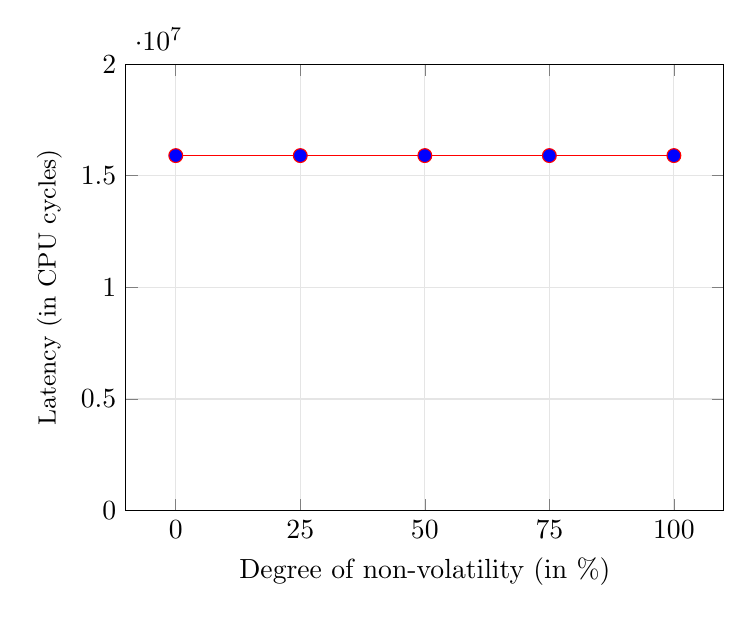
\begin{tikzpicture}
 
\begin{axis}[
	xmin = -10,
	xmax = 110,
	xtick distance = 25,
	ymin = 0,
	ymax = 20000000,
	ytick distance = 5000000,
    grid = both,
    major grid style = {gray!20},
    width = \columnwidth,
    height = 0.78\textwidth,
    xlabel = { \normalsize Degree of non-volatility (in \%)},
    ylabel = {\small Latency (in CPU cycles)},
    scale = 0.72
    ]

\addplot[red,mark=*,mark options={scale=1.25, fill=blue},text mark as node=true,point meta=explicit symbolic] coordinates { (0,15904185) (25,15904185) (50,15904185) (75,15904185) (100,15904185)};

\end{axis}
\end{tikzpicture}
	\end{subfigure}
	\begin{subfigure}{0.475\textwidth}
		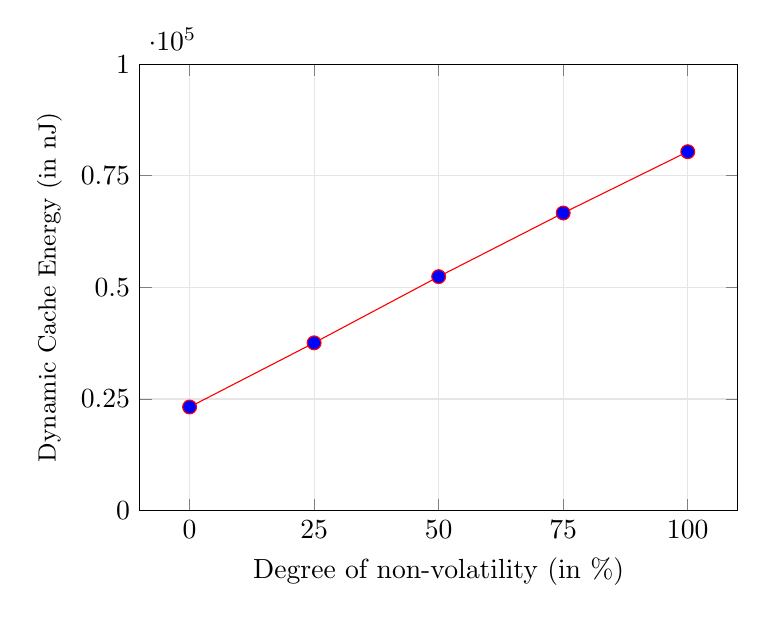
\begin{tikzpicture}
 
\begin{axis}[
	xmin = -10,
	xmax = 110,
	xtick distance = 25,
	ymin = 0,
	ymax = 100000,
	ytick distance = 25000,
    grid = both,
    major grid style = {gray!20},
    width = \columnwidth,
    height = 0.78\textwidth,
    xlabel = { \normalsize Degree of non-volatility (in \%)},
    ylabel = {\small Dynamic Cache Energy (in nJ)},
    scale = 0.72
    ]

\addplot[red,mark=*,mark options={scale=1.25, fill=blue},text mark as node=true,point meta=explicit symbolic] coordinates { (0,23217.578001) (25,37583.014876) (50,52414.414793) (75,66654.849654) (100,80393.959481)};

\end{axis}
\end{tikzpicture}
	\end{subfigure}
    \caption{Latency and dynamic energy consumption under different degrees of non-volatility for a write-intensive merge sort application.}
    \label{fig:FAUmsort}
\end{figure}

\begin{figure}
	\begin{subfigure}{0.475\textwidth}
		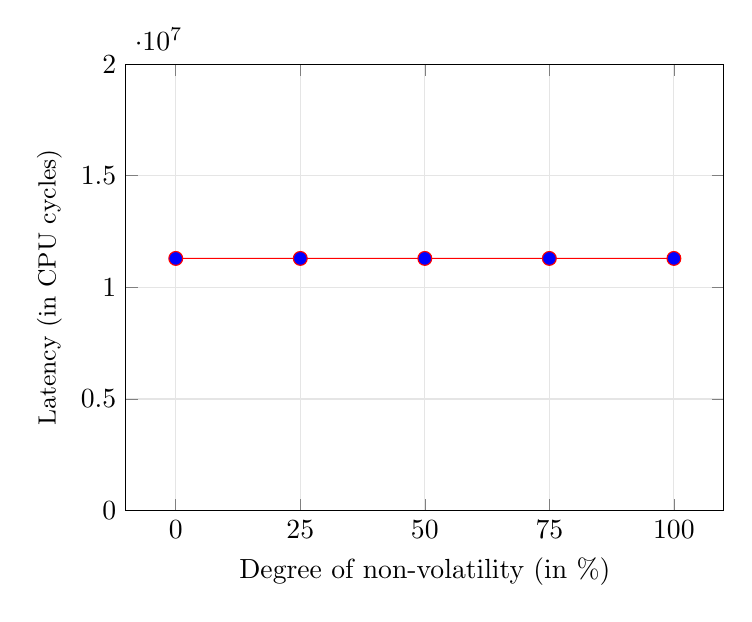
\begin{tikzpicture}
 
\begin{axis}[
	xmin = -10,
	xmax = 110,
	xtick distance = 25,
	ymin = 0,
	ymax = 20000000,
	ytick distance = 5000000,
    grid = both,
    major grid style = {gray!20},
    width = \columnwidth,
    height = 0.78\textwidth,
    xlabel = { \normalsize Degree of non-volatility (in \%)},
    ylabel = {\small Latency (in CPU cycles)},
    scale = 0.72
    ]

\addplot[red,mark=*,mark options={scale=1.25, fill=blue},text mark as node=true,point meta=explicit symbolic] coordinates { (0,11298120) (25,11298143) (50,11298143) (75,11298118) (100,11298118)};

\end{axis}
\end{tikzpicture}
	\end{subfigure}
	\begin{subfigure}{0.475\textwidth}
		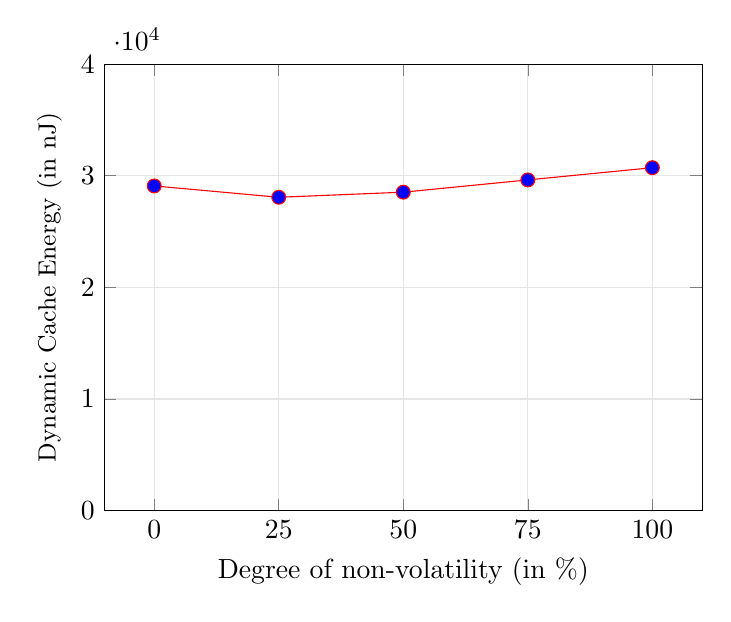
\begin{tikzpicture}
 
\begin{axis}[
	xmin = -10,
	xmax = 110,
	xtick distance = 25,
	ymin = 0,
	ymax = 40000,
	ytick distance = 10000,
    grid = both,
    major grid style = {gray!20},
    width = \columnwidth,
    height = 0.78\textwidth,
    xlabel = { \normalsize Degree of non-volatility (in \%)},
    ylabel = {\small Dynamic Cache Energy (in nJ)},
    scale = 0.72
    ]

\addplot[red,mark=*,mark options={scale=1.25, fill=blue},text mark as node=true,point meta=explicit symbolic] coordinates { (0,29088.925748) (25,28074.614715) (50,28530.362257) (75,29628.430611) (100,30723.784948)};

\end{axis}
\end{tikzpicture}
	\end{subfigure}
    \caption{Latency and dynamic energy consumption under different degrees of non-volatility for a read-intensive image processing application.}
    \label{fig:FAUip}
\end{figure}

\textit{Latency:} We can identify, that a higher degree of non-volatility barely influences the overall latency, despite the high NVM write latency.
This is explained by the fact, that in case of a cache write the CPU does not stall until the write is completed, unless data from the very same cache line is required in the meantime, which is rarely the case.

\textit{Dynamic Energy:} While the observation in the latency dimension holds for both applications, the dynamic energy under varying degrees of non-volatility behaves differently for the two applications.
For the write-intensive merge sort application, displayed in \cref{fig:FAUmsort}, the dynamic energy consumption rises proportionally with the increased degree of non-volatility.
This is to be expected, as the higher degree of non-volatility also implies a higher number of high energy NVM writes.
However, this is not the case for the image processing experiment, as seen in \cref{fig:FAUip}.
Here, as the application is highly read-intensive with read accesses in STT-RAM being more energy efficient than in SRAM, introducing NVM to a low degree can even reduce the dynamic energy consumption of the cache.
Using the toolchain with our hybrid cache extensions, we can thus analyze in which application scenarios and to which degree the introduction of NVM to the cache hierarchy proves the most beneficial.
Furthermore, for this case study, no replacement policies that consider the characteristics of the underlying memory technologies were analyzed.
These policies performing placement decisions according to, e.g., the predicted write intensity of future accesses, can further boost the performance of hybrid caches to a notable degree \cite{8716297,7110550, Wilbert:2024a}.

\subsubsection{Step-by-Step Instructions}
In the following we will provide a step-by-step guide on how hybrid caches are implemented in gem5.
First, we will create a \texttt{HybridCache} \texttt{SimObject} by inheriting the base methods from gem5's base cache class located in \texttt{src/mem/cache/base.cc}.
To account for the hybrid cache's asymmetric read/write latencies, we add additional parameters for the read and write latency of the non-volatile STT-RAM section.
Additionally, in order to generate meaningful statistics that allow for the analysis of hybrid caches, we add statistics for the dynamic energy consumption and number of accesses per section.
The gem5 \texttt{CacheBlk}, representing a cache line, is extended to a \texttt{HybridCacheBlk}, carrying the additional information whether the cache line is considered to be implemented in a volatile or non-volatile manner.
Whenever a cache line is accessed in the extended base cache class, we check for the volatility of the corresponding \texttt{HybridCacheBlk}.
Depending on whether the cache line is volatile or not, we thus take the latency and energy parameters for the SRAM or the STT-RAM section, respectively, as seen in the following listing where we exemplarily display the code for setting the latency and logging statistics following a write access to the hybrid cache.
\begin{lstlisting}[language=C]
HybridCacheBlk* hyblk = dynamic_cast<HybridCacheBlk*>(blk);
Cycles lat = hyblk->isVolatile() ? dataLatency : dataWriteLatency;
if (hyblk->isVolatile()) {
	hybrid_stats.noOfVolWrites++;
	hybrid_stats.dynEnergy += volWriteEnergy;
} else {
	hybrid_stats.noOfNonVolWrites++;
	hybrid_stats.dynEnergy += nonVolWriteEnergy;
}
\end{lstlisting}
The cache lines themselves are initialized and managed in the \texttt{BaseTags} class located in \texttt{src/mem/cache/tags/base.cc}.
To set the cache lines as volatile/non-volatile in accordance to the previously described \texttt{nvBlockRatio} parameter, we set the \texttt{HybridCacheBlk}'s volatile flag in the \texttt{HybridSetAssoc} class, which is derived from the \texttt{BaseTags} class.
\begin{lstlisting}[language=C]
int numNvBlocksPerSet = (nvBlockRatio/100)*assoc;
int numNvBlocksInSet = 0;
// Initialize all blocks
for (int blk_index = 0; blk_index < numBlocks; blk_index++) {
    HybridCacheBlk* blk = &blks[blk_index];
    if (blk_index 
        numNvBlocksInSet = 0;
    // Set whether block is volatile or non-volatile
    if (numNvBlocksInSet < numNvBlocksPerSet) {
        blk->setVolatile(false);
        numNvBlocksInSet++;
    } else {
        blk->setVolatile(true);
    }
}
\end{lstlisting}
On the Python configuration level in \texttt{configs/common/Caches.py}, we can define, e.g., L1 Data Caches as shown below, which are derived from the introduced \texttt{HybridCache} class, with hybrid-cache-specific parameters set to any desired value.
\begin{lstlisting}[language = Python]
class L1DCache(HybridCache):
    assoc = 4
    nv_block_ratio = 50
    data_read_latency = 2
    data_write_latency = 8
    ...
\end{lstlisting}
The connection between the C++ \texttt{SimObjects} containing the functional implementation and the Python classes setting a configuration is realized in \texttt{src/mem/cache/Cache.py} as follows.
\begin{lstlisting}[language = Python]
class HybridCache(ClockedObject):
    type = 'HybridCache'
    cxx_header = 'mem/cache/hybrid_cache.hh'
    cxx_class = 'gem5::HybridCache'
    data_read_latency = Param.Cycles("Data read access latency")
    data_write_latency = Param.Cycles("Data write access latency")
    ...
\end{lstlisting}
Furthermore, the additional hybrid-cache-specific parameters which can be set in the configuration files are named here.
For the \texttt{HybridSetAssoc} class, this is performed analogously in the \texttt{src/mem/cache/tags/Tags.py} file.
By running a gem5 simulation with Cache \texttt{SimObjects} of the \texttt{HybridCache} type, the analysis of heterogeneous cache architectures is thus made possible.
See \cref{app:fau}, for a more detailed description of the concrete command to perform and evaluate a simulation run.
\begin{insightbox}
In this case study, we have learned how gem5 can be extended to support caches incorporating both SRAM and STT-RAM cells.
We have observed in the experiments, that the write latency overhead of STT-RAM is barely noticeable in application scenarios.
While the introduction of NVM inherently lowers static power consumption in caches, even under conventional replacement policies, hybrid caches can further reduce dynamic energy consumption, depending on the characteristics of the application.
Owing to gem5's flexibility, our extension thus provides the opportunity to quickly evaluate the potential of hybrid caches when developing novel cache policies or investigating novel use-cases.

\end{insightbox}
